\documentclass{article}
\usepackage[utf8]{inputenc}
\usepackage{amsmath}
\usepackage{xcolor}
\usepackage[top=2cm, bottom=2cm, left=2cm, right=2cm]{geometry}
\setlength\parindent{0pt}

\usepackage{listings}
%\usepackage{color}
\usepackage{graphicx}
\usepackage{float}
\usepackage{caption}

\usepackage{verbatim}
\let\oldv\verbatim
\let\oldendv\endverbatim

%\userpackage{minted}

\definecolor{dkgreen}{rgb}{0,0.6,0}
\definecolor{gray}{rgb}{0.5,0.5,0.5}
\definecolor{mauve}{rgb}{0.58,0,0.82}
\definecolor{light-gray}{gray}{0.95}


\lstset{frame=tb,
  language=Java,
  aboveskip=6mm,
  belowskip=6mm,
  showstringspaces=false,
  columns=flexible,
  basicstyle={\small\ttfamily},
  numbers=none,
  numberstyle=\tiny\color{gray},
  keywordstyle=\color{blue},
  commentstyle=\color{dkgreen},
  stringstyle=\color{mauve},
  breaklines=true,
  breakatwhitespace=true,
  tabsize=3,
  backgroundcolor=\color{light-gray},
  language=Matlab
}

%\usepackage{natbib} replaced by line below to make refernces work
\usepackage[square,sort,comma,numbers]{natbib}
\usepackage[nottoc,numbib]{tocbibind} %to get references in table of contants
\usepackage{graphicx}

\usepackage{bm}

\usepackage{hyperref}
\hypersetup{
	colorlinks,
	citecolor=black,
	filecolor=black,
	linkcolor=black,
	urlcolor=black
}

\usepackage{mdframed}
\usepackage{lipsum} % for creating dummy text
\mdfdefinestyle{MyFrame}{%
	linecolor=black,	
	backgroundcolor=gray!20!white,
	skipbelow = 8mm,
	skipabove = 8mm}

\usepackage{scrextend}

\title{Fys4150\\Project 1\\ }
\author{Peter Killingstad and Karl Jacobsen}


\begin{document}
	
\maketitle

\tableofcontents

\pagebreak
\section{Abstract}

\section{Introduction}
Goals: Learn C++, dynamic memory allocation, discretizing differential equations and setting up a linear system, algorithms for solving tridiagonal linear systems, error-analysis (truncation and precision), efficiency analysis.

\section{Theory}


\subsection{Setting up the linear system}
In this project we will solve the one-dimensional Poisson equation
with Dirichlet boundary conditions by rewriting it as a set of linear equations.


To be more explicit we will solve the equation

\begin{equation*}
-u''(x) = f(x), \hspace{0.5cm} x\in(0,1), \hspace{0.5cm} u(0) = u(1) = 0.
\end{equation*}
and we define the discretized approximation  to $u$ as $v_i$  with 
grid points $x_i=ih$   in the interval from $x_0=0$ to $x_{n+1}=1$.
The step length or spacing is defined as $h=1/(n+1)$. 
We have then the boundary conditions $v_0 = v_{n+1} = 0$.
We  approximate the second
derivative of $u$ with

\begin{equation*}
-\frac{v_{i+1}+v_{i-1}-2v_i}{h^2} = f_i  \hspace{0.5cm} \mathrm{for} \hspace{0.1cm} i=1,\dots, n,
\end{equation*}
where $f_i=f(x_i)$. \\

Now we will show that the discrete problem can be rewritten to a linear system of the type 

\begin{equation*}
\mathbf{A}\mathbf{v} = \tilde{\mathbf{b}}.
\end{equation*}

The reason for wanting the rewrite to a linear system, is that we know of methods that solve such linear systems. Hence, by solving the linear system we will also solve our discrete differential eauquation problem!\\

\textbf{Task 1} We get to the linear system by setting in the first couple of values in the above equation with v's, and notice the pattern. 

\subsection{Gaussian elimination tridiagonal systems}
We use standard Gaussian elimination, utlizing the sparsity of the matrix by ignoring the zero terms when doing the forward and backward substitution. This gives the Thomas algorithm. The algorithm can be seen in our code, which follows:

\begin{lstlisting}
void gaussianTridiagonalSolver(double ** computed_tridiagonal_matrix, double * computed_right_hand_side, double * computed_numerical_solution, int N){
double multiplicationFactor;
for (int i = 1; i < N; i++){
multiplicationFactor = computed_tridiagonal_matrix[i][i-1]/computed_tridiagonal_matrix[i-1][i-1];
computed_tridiagonal_matrix[i][i-1] = 0;
computed_tridiagonal_matrix[i][i] += - multiplicationFactor*computed_tridiagonal_matrix[i-1][i];
computed_right_hand_side[i] += - multiplicationFactor*computed_right_hand_side[i-1];
}
for(int i = N-1; i > -1; i--){
if(i == N-1)
computed_numerical_solution[i] = computed_right_hand_side[i];
else
computed_numerical_solution[i] = computed_right_hand_side[i+1] - computed_tridiagonal_matrix[i][i+1]*computed_numerical_solution[i+1]/computed_tridiagonal_matrix[i][i];
}

}
\end{lstlisting}

\textbf{Task 2} We can insert a few comments in the top of the function, explaining the algorithm. \\

Now we want to calculate the number of floating points operations (FLOPS) needed to solve the linear system with the above algorithm. This is an extremely important topic, since the number of FLOPS typically will be very large in physics problems, and having an algorithm that reduces the FLOPS can be the difference between being able to solve the problem and not!\\

\textbf{Task 3} Here we must do, and show, the calculations of FLOPS in our algorithm. It should, according to Wikipedia, be $\mathcal{O}(n)$ FLOPS.

\subsection{Gaussian elimination symmetric tridiagonal systems}
If the tridiagonal system is symmetric, $A = A^T$, the Gaussian elimination method can be made even simpler than in the Thomas algorithm. The program below shows the algorithm and its implementation.

\begin{lstlisting}
void gassianTridiagonalSymmetricSolver(double ** computed_tridiagonal_matrix, double * computed_right_hand_side, double * computed_numerical_solution, int N){
for (int i = 1 ; i < N; i++){
computed_tridiagonal_matrix[i][i] += -computed_tridiagonal_matrix[i-1][i]*computed_tridiagonal_matrix[i-1][i]/computed_tridiagonal_matrix[i-1][i-1];
computed_right_hand_side[i] += -computed_tridiagonal_matrix[i-1][i]*computed_right_hand_side[i-1]/computed_tridiagonal_matrix[i-1][i-1];
}

computed_numerical_solution[N-1] = computed_right_hand_side[N-1]/computed_tridiagonal_matrix[N-1][N-1];
for (int i = N-2; i > -1; i--){
computed_numerical_solution[i] = computed_right_hand_side[i] - computed_tridiagonal_matrix[i][i+1]*computed_numerical_solution[i+1]/computed_tridiagonal_matrix[i+1][i+1];
}
}
\end{lstlisting}

\textbf{Task 4} The above listing must be made more pretty bby fixing the spaces, but that can wait tuil we know we have the final program. Also for this function, we should in the top add lines describing the algorithm.\\

\textbf{Task 5} Here we should do, and show, FLOP-count for the above listed algorithm.

\subsection{Error calculations}
Having knowledge about the errors of the numerical solutions is essential, because without this knowledge, it is difficult to know the validity of the results. Without knowledge of validity of the results, we are exiting the subject of (natural) science. \\

In our differential equation, we approximate the 2nd derivative with a truncated Taylor-polynomial. A nice thing by using Taylor ploynomials is that we have knowledge about the truncation error, the difference between numerical and exact solution due to terms in the Taylor series being left out. It turns out that in our case the truncation error depends on the step size, $h$. Hence we know what to expect of the truncation error when varying $h$. \\

In our case the truncation error is of $\mathcal{O}(h^2)$. From this we expect the truncation error to depend on the step lenght, $h$, to a order of 2, meaning that a reduction of $h$ by a factor of 10 should reduce the truncation error by a factor of 20.\\

We are more interested in the relative error, meaning the difference between the numerical and exact solution, relateive to the exact solution, than in the pure error. The reason for this, is that a small pure error could be physically insignificant if the quantities are big, while on the other hand a small pure error could be very significant if the quantities we are measuring are small. Example: 1 cm in error when simulating trajectories of planets is probably less physically significant than 1 cm error when doing simulations on molecular level.\\

For inspection of errors, and relating them to the expected convergence rates from Taylor series theory, it is neat to take the log the the errors and of the step lengths. Plotting this, the slopes could be directly compared with the expected convergence rate, the $\mathcal{O}$-term from the Taylor approximation of the 2nd derivative.\\

Our solutions will be vectors, so there will be errors at each vector element. We are interested in a rough error-number, so we want an error measure that represents all of the array-points. One way of doing this, is for each step length to extract the max value of the relative error. By this method, we know that the error we get is an upper bound for all local errors, local meaning errors at the different vector elements.\\

By the methods mentioned above, we compute the relative error in the data set $i=1,\dots, n$,by setting up

\[
\epsilon_i=log_{10}\left(\left|\frac{v_i-u_i}
{u_i}\right|\right),
\]
as function of $log_{10}(h)$ for the function values $u_i$ and $v_i$, and extract the maximum for each step length.\\

As an alternative we also computed the L2-error norm, which basically sums up all the local errors to one single measure. The reason for also including this norm, is that it can give some extra information about the overall performance of the numerical approximation over the whole domain.

\subsection{LU}
We will compare the speed of our algorithms with the speed of the LU-algorithm. According to Hjorth-Jensen \cite{MHJ} p. 173, solving a system with LU is $\mathcal{O}(n^2)$ requires FLOPS, but the composition itself requires  $\mathcal{O}(n^3)$ FLOPS. Based on this, we expect our algorithms to outperform the LU-algorithm, independentlyu of whether one includes the composition itself in the comparison or not.\\

\textbf{Task 6} Insert code for importing LU from Armadillo and the commands used.

\section{Results}

\subsection{Thomas algorithm}
\textbf{Task 7} Comment on the figure.

\begin{figure}[H]
	\centering
	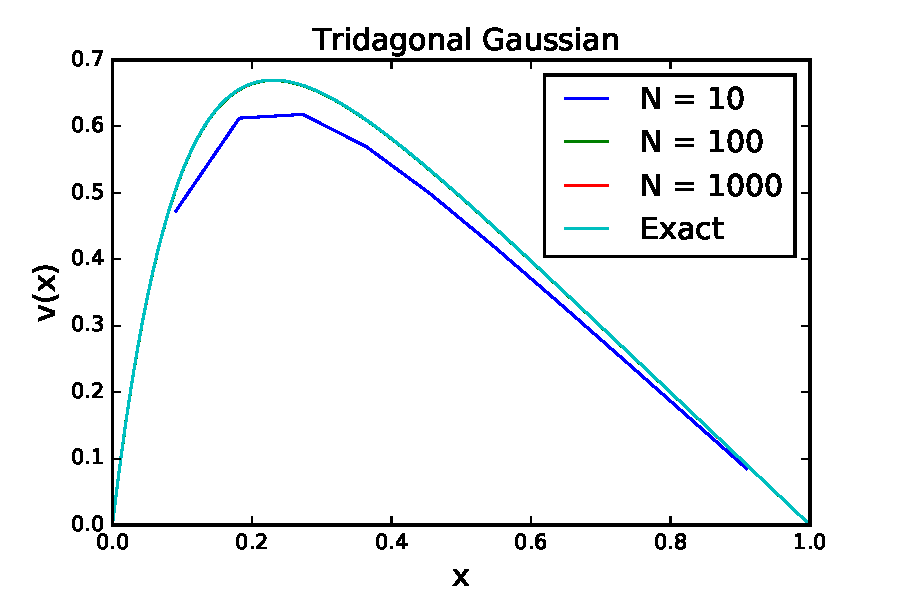
\includegraphics[width=0.99\textwidth]{/home/karl/doc/subj/att/fys4150/build-project1qt-Desktop_Qt_5_9_1_GCC_64bit-Debug/gaussianTridiagonal_comparison.pdf}
	\caption{Results Tridiagonal Gaussian}
	%\label{1}
\end{figure}

\subsection{Symmetric vs Thomas}


\lstset{backgroundcolor=\color{white}}
\begin{minipage}{.49\textwidth} %\noindent
	\lstinputlisting[language={},title={Tridiagonal
	}]{/home/karl/doc/subj/att/fys4150/project1/cpuTimeTridiagonal.tex}
\end{minipage}\hfill
\begin{minipage}{.49\textwidth}
	\lstinputlisting[language={},title={Symmetric
	}]{/home/karl/doc/subj/att/fys4150/project1/cpuTimeSymmetric.tex}
\end{minipage}\hfill



\subsection{Error}
\begin{minipage}{.49\textwidth} %\noindent
\begin{figure}[H]
	\centering
	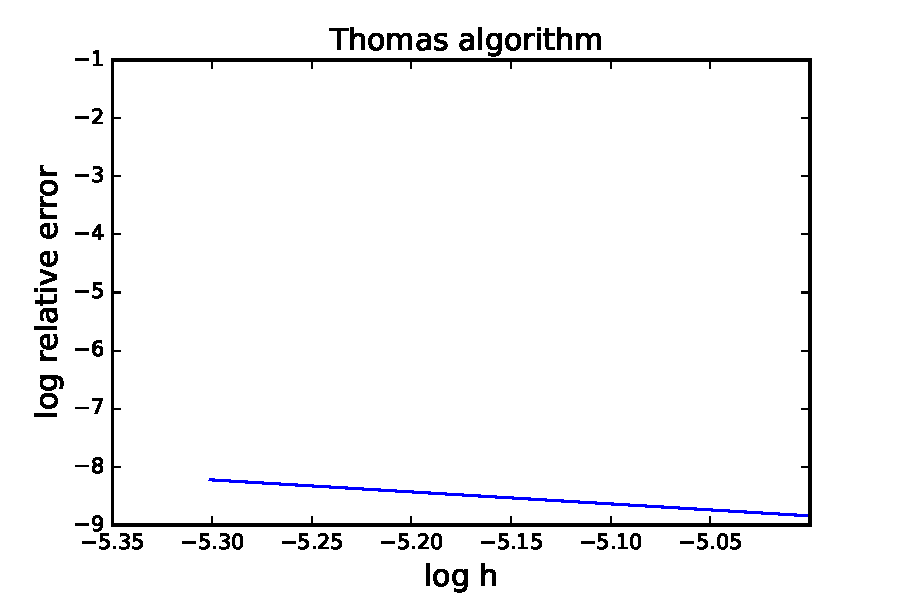
\includegraphics[width=0.99\textwidth]{/home/karl/doc/subj/att/fys4150/build-project1qt-Desktop_Qt_5_9_1_GCC_64bit-Debug/gaussianTridiagonal_error2.pdf}
	\caption{Results Tridiagonal Gaussian}
	%\label{1}
\end{figure}
\end{minipage}\hfill
\begin{minipage}{.49\textwidth}
\begin{figure}[H]
	\centering
	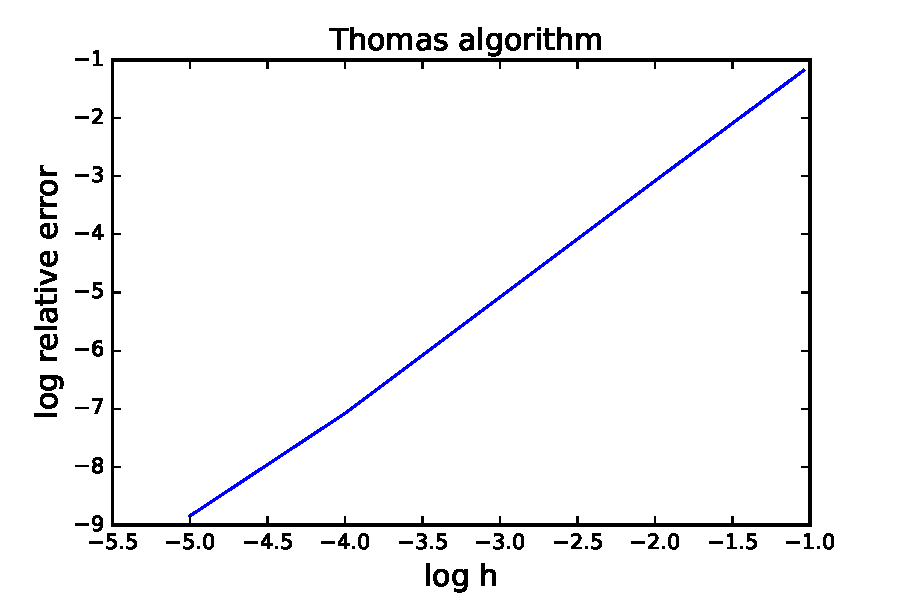
\includegraphics[width=0.99\textwidth]{/home/karl/doc/subj/att/fys4150/build-project1qt-Desktop_Qt_5_9_1_GCC_64bit-Debug/gaussianTridiagonal_error.pdf}
	\caption{Results Tridiagonal Gaussian}
	%\label{1}
\end{figure}

\end{minipage}\hfill




Our computer crashes for $N = 10^6$, so the above figure to the right stops at $N = 10^5$. The figure shows that up to $N = 10^5$, the error seems to follow the expected truncation error, since the slope seems to be pretty close to 2.\\

The figure to the left above shows the error-development staring where the previous figure left off, but with smaller increases in $N$.


\subsection{LU}
\textbf{Task 10} We compare the cpu time for LU with the CPU-times for the other two algorithms, for $N=10, 100, 1000$. \\

\textbf{Task 11} Copmute error for $N=1000$ for LU and one of the other two algorithms. The results should be identical.

\textbf{Task 12} LU possible $N=10^5$? Find out.

\section{Conclusions}
\textbf{Task 13} Sum up the results here.

\section{Feedback}
\textbf{Task 14} What has been good, something that could have been done better?

\begin{thebibliography}{9}
	\bibitem{MHJ} 
	Hjorth-Jensen, M.(2015)
	\textit{Computational physics. Lectures fall 2015}. 
	\url{https://github.com/CompPhysics/ComputationalPhysics/tree/master/doc/Lectures}
\end{thebibliography}


\end{document}